\section{configobj::Config\-Obj Class Reference}
\label{classconfigobj_1_1ConfigObj}\index{configobj::ConfigObj@{configobj::ConfigObj}}
Inheritance diagram for configobj::Config\-Obj::\begin{figure}[H]
\begin{center}
\leavevmode
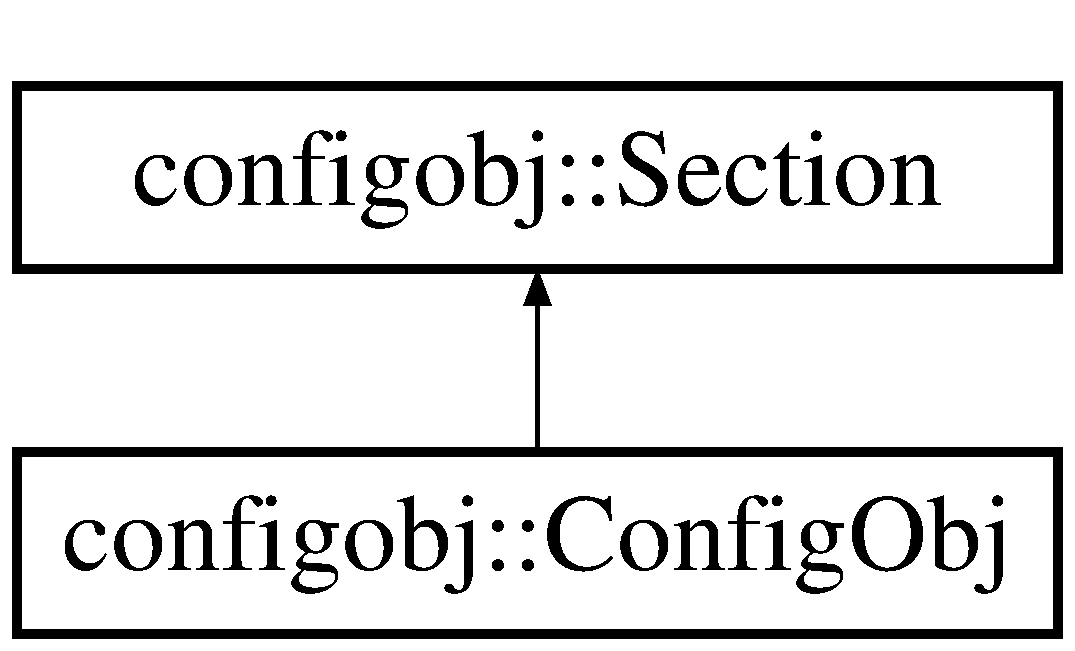
\includegraphics[height=2cm]{classconfigobj_1_1ConfigObj}
\end{center}
\end{figure}
\subsection*{Public Member Functions}
\begin{CompactItemize}
\item 
def {\bf\_\-\_\-init\_\-\_\-}
\item 
def \textbf{\_\-\_\-repr\_\-\_\-}\label{classconfigobj_1_1ConfigObj_e0d8b19d3f755c83604f4e2c1027fa05}

\item 
def {\bfwrite}
\item 
def {\bfvalidate}
\end{CompactItemize}


\subsection{Detailed Description}


\footnotesize\begin{verbatim}An object to read, create, and write config files.\end{verbatim}
\normalsize
 



\subsection{Member Function Documentation}
\index{configobj::ConfigObj@{configobj::Config\-Obj}!__init__@{\_\-\_\-init\_\-\_\-}}
\index{__init__@{\_\-\_\-init\_\-\_\-}!configobj::ConfigObj@{configobj::Config\-Obj}}
\subsubsection{\setlength{\rightskip}{0pt plus 5cm}def configobj::Config\-Obj::\_\-\_\-init\_\-\_\- ( {\em self},  {\em infile} = {\tt None},  {\em options} = {\tt None},  {\em kwargs})}\label{classconfigobj_1_1ConfigObj_6f3d2c0ab8c49831b35389fa805417b2}




\footnotesize\begin{verbatim}
Parse or create a config file object.

``ConfigObj(infile=None, options=None, **kwargs)``
\end{verbatim}
\normalsize
 \index{configobj::ConfigObj@{configobj::Config\-Obj}!write@{write}}
\index{write@{write}!configobj::ConfigObj@{configobj::Config\-Obj}}
\subsubsection{\setlength{\rightskip}{0pt plus 5cm}def configobj::Config\-Obj::write ( {\em self},  {\em outfile} = {\tt None},  {\em section} = {\tt None})}\label{classconfigobj_1_1ConfigObj_60722dd8c38412b05cab80755298187d}




\footnotesize\begin{verbatim}
Write the current ConfigObj as a file

tekNico: FIXME: use StringIO instead of real files

>>> filename = a.filename
>>> a.filename = 'test.ini'
>>> a.write()
>>> a.filename = filename
>>> a == ConfigObj('test.ini', raise_errors=True)
1
\end{verbatim}
\normalsize
 \index{configobj::ConfigObj@{configobj::Config\-Obj}!validate@{validate}}
\index{validate@{validate}!configobj::ConfigObj@{configobj::Config\-Obj}}
\subsubsection{\setlength{\rightskip}{0pt plus 5cm}def configobj::Config\-Obj::validate ( {\em self},  {\em validator},  {\em preserve\_\-errors} = {\tt False},  {\em copy} = {\tt False},  {\em section} = {\tt None})}\label{classconfigobj_1_1ConfigObj_c5c1180a0065104014f50d37a7d0852c}




\footnotesize\begin{verbatim}
Test the ConfigObj against a configspec.

It uses the ``validator`` object from *validate.py*.

To run ``validate`` on the current ConfigObj, call: ::

    test = config.validate(validator)

(Normally having previously passed in the configspec when the ConfigObj
was created - you can dynamically assign a dictionary of checks to the
``configspec`` attribute of a section though).

It returns ``True`` if everything passes, or a dictionary of
pass/fails (True/False). If every member of a subsection passes, it
will just have the value ``True``. (It also returns ``False`` if all
members fail).

In addition, it converts the values from strings to their native
types if their checks pass (and ``stringify`` is set).

If ``preserve_errors`` is ``True`` (``False`` is default) then instead
of a marking a fail with a ``False``, it will preserve the actual
exception object. This can contain info about the reason for failure.
For example the ``VdtValueTooSmallError`` indeicates that the value
supplied was too small. If a value (or section) is missing it will
still be marked as ``False``.

You must have the validate module to use ``preserve_errors=True``.

You can then use the ``flatten_errors`` function to turn your nested
results dictionary into a flattened list of failures - useful for
displaying meaningful error messages.
\end{verbatim}
\normalsize
 

The documentation for this class was generated from the following file:\begin{CompactItemize}
\item 
old/PANICtool-1.0/configobj.py\end{CompactItemize}
